\documentclass[preprint,12pt,a4paper]{elsarticle}

\usepackage[utf8]{inputenc}
\usepackage{amsmath,amssymb}
\usepackage{booktabs}
\usepackage{array}
\usepackage{graphicx}
\usepackage{xcolor}
\usepackage{hyperref}
\usepackage{xurl}
\usepackage{caption}
\usepackage{subcaption}
\usepackage{float}
\usepackage{placeins}
\usepackage{microtype}

\journal{SoftwareX}

\captionsetup{font=small,labelfont=bf,skip=4pt}
\captionsetup[sub]{font=scriptsize,labelfont=bf}
\raggedbottom

% =====================================================================
% Float placement tuning: keep text flowing and avoid large white gaps.
% [H] forces a float exactly here and leaves blank space at the bottom
% of a page when the float will not fit. Below we switch every float to
% [htbp] and let LaTeX fill more of each page with floats before it
% gives up and emits a sparse float page.
% =====================================================================
\renewcommand{\topfraction}{0.92}        % up to 92% of a page top may be floats
\renewcommand{\bottomfraction}{0.92}     % up to 92% of a page bottom may be floats
\renewcommand{\textfraction}{0.06}       % at least 6% of a float page must be text
\renewcommand{\floatpagefraction}{0.75}  % a float-only page must be >=75% full
\setcounter{topnumber}{4}
\setcounter{bottomnumber}{4}
\setcounter{totalnumber}{8}
\setlength{\textfloatsep}{8pt plus 2pt minus 2pt}
\setlength{\floatsep}{8pt plus 2pt minus 2pt}
\setlength{\intextsep}{8pt plus 2pt minus 2pt}
\setlength{\abovecaptionskip}{3pt}
\setlength{\belowcaptionskip}{2pt}
\makeatletter
\setlength{\@fptop}{0pt}
\setlength{\@fpsep}{8pt plus 2pt minus 2pt}
\setlength{\@fpbot}{0pt plus 1fil}
\makeatother

\hypersetup{
  colorlinks=true,
  linkcolor=blue!50!black,
  citecolor=blue!50!black,
  urlcolor=blue!50!black
}

\graphicspath{{figures/}}

\begin{document}

\begin{frontmatter}

\title{FRACMATH: A vectorized MATLAB framework for continuum damage
mechanics with crack band regularization}

\author[unm]{Jaykumar~Mavani}
\author[unm]{Madura~Pathirage\corref{cor1}}
\ead{mpathirage@unm.edu}
\cortext[cor1]{Corresponding author}
\address[unm]{Gerald May Department of Civil, Construction, and Environmental Engineering,
University of New Mexico, Albuquerque, NM, USA}

\begin{abstract}
\texttt{FRACMATH} is an open-source MATLAB framework for the finite element
simulation of fracture in concrete and other quasibrittle materials. The
software implements scalar isotropic continuum damage mechanics with the
modified von Mises equivalent strain, exponential softening, and crack-band
regularization based on a direction-dependent Oliver characteristic length,
and solves quasistatic problems in 2D and 3D with a vectorized modified
Newton--Raphson scheme. The package ships with benchmark input decks,
plotting scripts, an Abaqus/Standard UMAT, and a documented comparison
workflow. In the principal validation case, a notched two-dimensional
three-point bending benchmark, the MATLAB solver reproduces the
Oliver-matched Abaqus UMAT peak load within 1\% while completing the run
about 3.6 times faster. Two further three-dimensional examples, the
Nooru-Mohamed mixed-mode test and the Brokenshire torsion demonstration,
show curved and nonplanar crack paths. Source code, benchmarks, and a theory
manual are released under the MIT license.
\end{abstract}

\begin{keyword}
continuum damage mechanics \sep crack-band regularization \sep finite
element method \sep MATLAB \sep Abaqus UMAT \sep quasibrittle fracture
\end{keyword}

\end{frontmatter}

% =====================================================================
\section*{Required Metadata}
\label{sec:metadata}
% =====================================================================

\section*{Current code version}
\label{sec:current-code-version}

\begin{table}[H]
\centering
\begin{tabular}{|l|p{5.5cm}|p{6.8cm}|}
\hline
\textbf{Nr.} & \textbf{Code metadata description} & \textbf{Value} \\
\hline
C1 & Current code version & v1.0.0 \\
\hline
C2 & Permanent GitHub link to code/repository used for this code version &
\url{https://github.com/Jaykumar9033/FRACMATH/tree/v1.0.0} \\
\hline
C3 & Legal Code License & MIT License \\
\hline
C4 & Code versioning system used & git \\
\hline
C5 & Software code languages, tools, and services used & MATLAB, Fortran
UMAT, Abaqus/Standard, Python plotting scripts \\
\hline
C6 & Compilation requirements, operating environments \& dependencies &
MATLAB R2022a or newer for the MATLAB solver; Abaqus/Standard 2023 for
the UMAT comparison; Python 3 for plotting and post-processing scripts \\
\hline
C7 & If available Link to developer documentation/manual &
Repository README, reproducibility guide, and theory manual in the
GitHub repository \\
\hline
C8 & Support email for questions & \href{mailto:mpathirage@unm.edu}{mpathirage@unm.edu} \\
\hline
\end{tabular}
\caption{Code metadata.}
\label{tab:code-metadata}
\end{table}

% =====================================================================
\section*{Motivation and significance}
% =====================================================================

\texttt{FRACMATH} is an open source MATLAB framework for finite element
simulation of fracture in quasibrittle materials. It uses scalar
isotropic continuum damage mechanics (CDM) built on the modified von
Mises equivalent strain measure \citep{deVree}, exponential softening,
and crack band regularization through a characteristic crack-band length
\citep{oliver1989,bazant_oh}. Quasistatic loading is solved with a
vectorized modified Newton--Raphson scheme under displacement control.

The package comes with three benchmark cases. The main benchmark is a
notched 2D three point bending (3PB) test of a concrete beam at a depth
of $D=100$~mm with a notch ratio of $a/D=0.2$, run in MATLAB and
checked against Abaqus/Standard with an Oliver-matched UMAT. Two more
cases run in MATLAB only: a 3D mixed mode Nooru-Mohamed validation test
and a 3D notched beam torsion demonstration.

Source code, documentation, and benchmark inputs live at
\url{https://github.com/Jaykumar9033/FRACMATH} under the MIT license.

% =====================================================================
\subsection*{Scientific need and related work}
% =====================================================================

CDM with crack band regularization is the usual way to run finite
element simulations of fracture in concrete and rock at the structural
scale \citep{bazant_planas}. The two mature tools in everyday research
use are Abaqus driven by a UMAT or VUMAT subroutine that the user writes
\citep{abaqus} and the C++ research code OOFEM \citep{oofem}. Both are
powerful but take real effort to learn for anyone not already writing
Fortran or modern C++. Adapting either
one to a new equivalent strain measure or an unusual arc length scheme
can eat up weeks of setup before the first curve worth reviewing appears.

MATLAB sits in nearly every engineering curriculum. It ships a sparse
direct solver that holds its own against anything else on small and
medium problems \citep{umfpack}, along with a profiler and a debugger
that most students already know. What has been missing is a complete
damage mechanics package that installs with no configuration, handles
both 2D and 3D meshes, and can be checked against an Abaqus UMAT on a
standard 3PB benchmark.

\texttt{FRACMATH} fills that gap. The reader we have in mind is a graduate
student or early career researcher who needs a damage simulation running
now and results worth publishing soon after. A second audience is
structural engineers who want a transparent reference implementation
when they check commercial code. CALFEM \citep{calfem} is popular for
teaching but carries no damage models and no crack band regularization.
To our knowledge, no other open source MATLAB package offers a complete
damage solver with crack band regularization in both 2D and 3D together
with a documented Oliver-matched Abaqus UMAT comparison for a standard
3PB benchmark.



% =====================================================================
\section*{Software description}
% =====================================================================

The formulation is standard, so we list only the key pieces here; the
full derivations are in the manual.

A scalar damage variable $\omega \in [0,1]$ degrades the elastic
stiffness,
$\boldsymbol{\sigma} = (1-\omega)\,\mathbb{C}_0:\boldsymbol{\varepsilon}$.
The history variable $\kappa(t)=\max_{\tau\le t}\tilde{\varepsilon}(\tau)$
tracks the largest equivalent strain ever reached, so damage cannot heal.
The equivalent strain follows the modified von Mises measure proposed by
de Vree et al. \citep{deVree},
\begin{equation}
\tilde{\varepsilon} = \frac{k-1}{2k(1-2\nu)}I_1
  + \frac{1}{2k}\sqrt{\left(\frac{k-1}{1-2\nu}\right)^2 I_1^2
  + \frac{12k}{(1+\nu)^2}J_2}
\end{equation}
where $k = f_c/f_t$ is the ratio of compressive to tensile strength.

Softening is exponential,
$\omega(\kappa) = 1 - (\kappa_0/\kappa)\exp[-(\kappa-\kappa_0)/(\varepsilon_f - \kappa_0)]$,
with $\kappa_0 = f_t/E$; the softening parameter $\varepsilon_f$ is
calibrated for each element so that the dissipated energy equals $G_F$.
Crack band regularization scales this softening branch to the element
size so that $G_F = h \cdot g_f$ holds whatever the mesh refinement
\citep{bazant_oh}. In the MATLAB implementation, the characteristic
length $h$ comes from Oliver's projected crack-band length
\citep{oliver1989}, computed from the element geometry and the local
principal strain direction at each integration point. For a three-node
triangle, the projected bandwidth is evaluated as
\begin{equation}
  h(\mathbf{n}) =
  \frac{2}{\sum_{a=1}^{3}|\nabla N_a \cdot \mathbf{n}|},
  \label{eq:oliver-t3}
\end{equation}
where $\mathbf{n}$ is the maximum principal strain direction. The same
projection idea is used for the 2D triangles and the 3D tetrahedra, so
the dissipation stays tied to the local crack direction rather than to a
fixed mesh direction.

For the Abaqus/Standard comparison of the 2D CPS3 model, the same
T3 formula in Eq.~\eqref{eq:oliver-t3} is used. An Abaqus UMAT does not
receive the complete element nodal geometry in the same convenient form
as the MATLAB element routine, so the Abaqus preprocessing script writes
the element shape-function gradients to
\texttt{oliver\_t3\_gradN.dat}. The UMAT reads this table and recomputes
$h(\mathbf{n})$ from the current maximum principal strain direction at
each material point. The Abaqus comparison thus uses the same direction-dependent Oliver bandwidth as the MATLAB solver,
rather than using the Abaqus characteristic element length
\texttt{CELENT} as the crack-band length.

Each load step is solved with a vectorized modified Newton Raphson
scheme. At a prescribed displacement increment, the solver assembles a
secant stiffness from the current damage state, factors the
free-degree-of-freedom block once, and reuses that factorization during
the equilibrium iterations. After the displacement correction converges,
stresses, strains, and damage variables are updated for all elements in
vectorized matrix operations through \texttt{pagemtimes}; the damaged
stiffness is then reassembled for the reaction force and for the next
load step. Linear systems go through MATLAB's \texttt{\textbackslash}
operator, which dispatches to UMFPACK \citep{umfpack}.

% =====================================================================
\section*{Illustrative examples}

\subsection*{Benchmark 1: Notched 2D Three Point Bending}
% =====================================================================

The specimen is a concrete beam following the Gr\'egoire geometry
\citep{gregoire2013}: depth $D = 100$~mm, support span
$S = 250$~mm (so $S/D = 2.5$), two overhangs of $0.5D$ each, and an
overall length of $350$~mm. The out-of-plane thickness is $50$~mm. A
single vertical notch is placed at midspan with an initial notch depth
$a_0 = 0.2D = 20$~mm and a notch width of $D/40 = 2.5$~mm. The geometry,
mesh, and boundary conditions are shown in Figure~\ref{fig:b1-setup-response}(a). The
material is concrete with $E = 37{,}000$~MPa, $\nu = 0.20$,
$f_t = 3.5$~MPa, $f_c = 35.0$~MPa, and $G_F = 0.090$~N/mm.

The mesh consists of CPS3 elements, i.e. three-node linear plane-stress
triangles. The same Abaqus-generated mesh is used by both solvers. It is
a free triangular mesh with local refinement in a rectangular zone of
width $D/2$ and height $D$ centred on the notch. The final mesh contains
14{,}268 CPS3 elements and 7{,}319 nodes, corresponding to 14{,}638
in-plane displacement degrees of freedom in the MATLAB run. Load is
applied under displacement control at the three top-edge nodes nearest
midspan, with a final vertical displacement of $-0.2$~mm. The left support
is pinned, the right support is a roller, and the crack mouth opening
displacement (CMOD) is computed as the horizontal displacement difference
between the two node sets on the notch mouth at $y=0$.

For the timing comparison, MATLAB R2024a was run in single-thread
mode and Abaqus/Standard 2023 was run using four threads. The timing
values reported below were measured on the development workstation
(Windows 11, Intel Core i9-13900, 64~GB RAM, NVMe SSD).

The simulated MATLAB peak load is 3.64~kN at a CMOD of
0.022811~mm. The Abaqus UMAT peak load is 3.61~kN at a CMOD of
0.022485~mm. The full load--CMOD response is shown in
Figure~\ref{fig:b1-setup-response}(b). The MATLAB and Abaqus curves agree closely
up to peak load. The two post-peak branches are similar in shape but not
identical; the remaining differences are attributed to the different
global solution procedures, convergence paths, increment histories, and
state-variable update order in MATLAB and Abaqus.

\begin{figure}[!htbp]
  \centering
  \begin{subfigure}{0.48\linewidth}
    \centering
    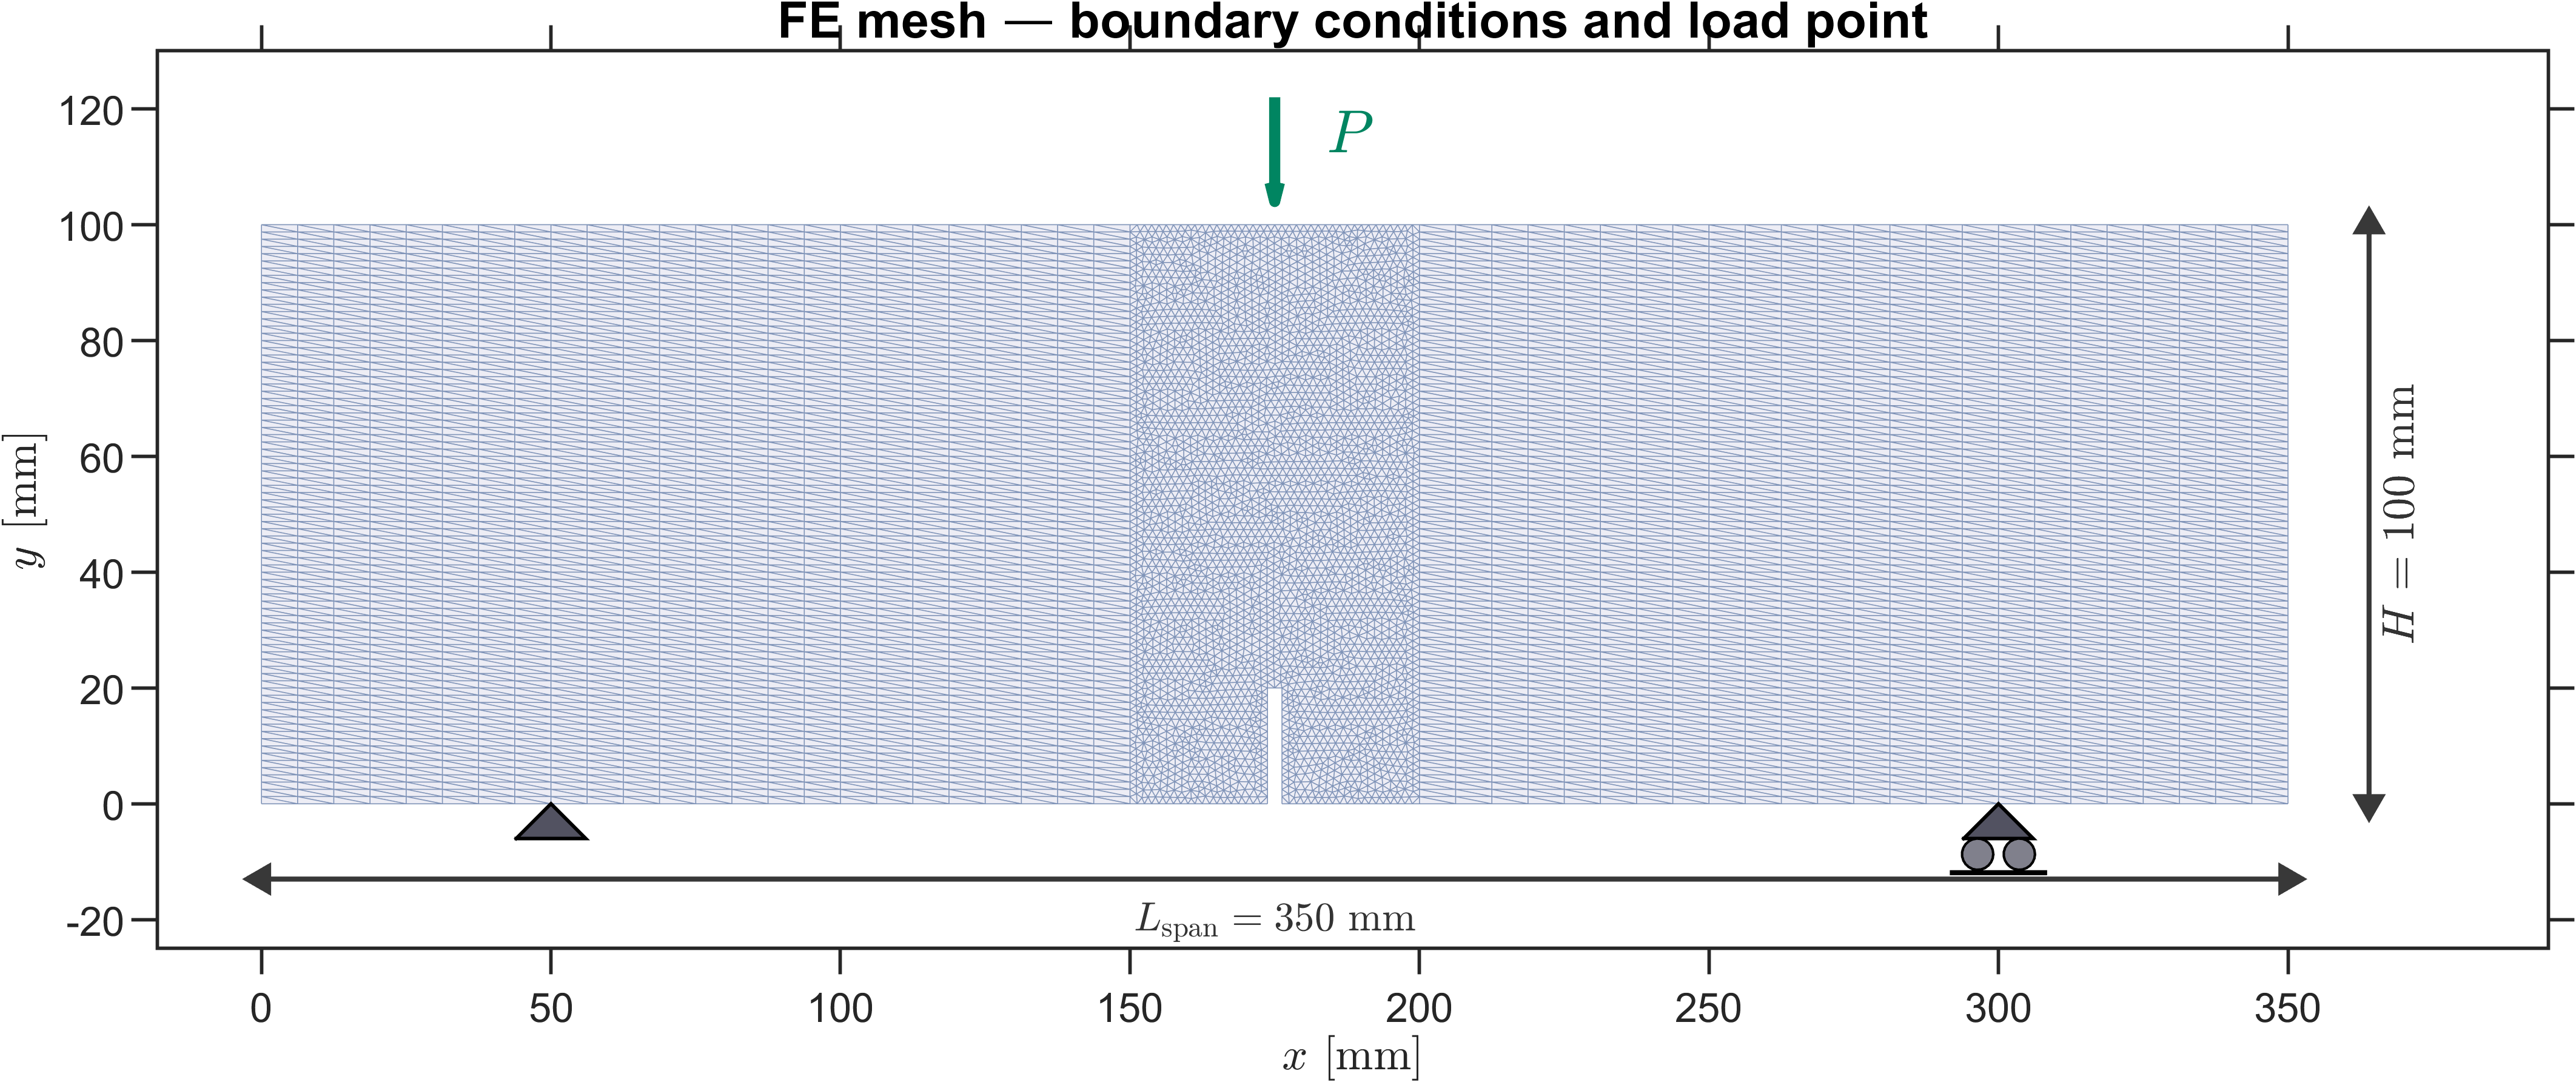
\includegraphics[width=\linewidth]{fig_mesh.png}
    \caption{Geometry, refined CPS3 mesh, supports, and load point.}
  \end{subfigure}
  \hfill
  \begin{subfigure}{0.48\linewidth}
    \centering
    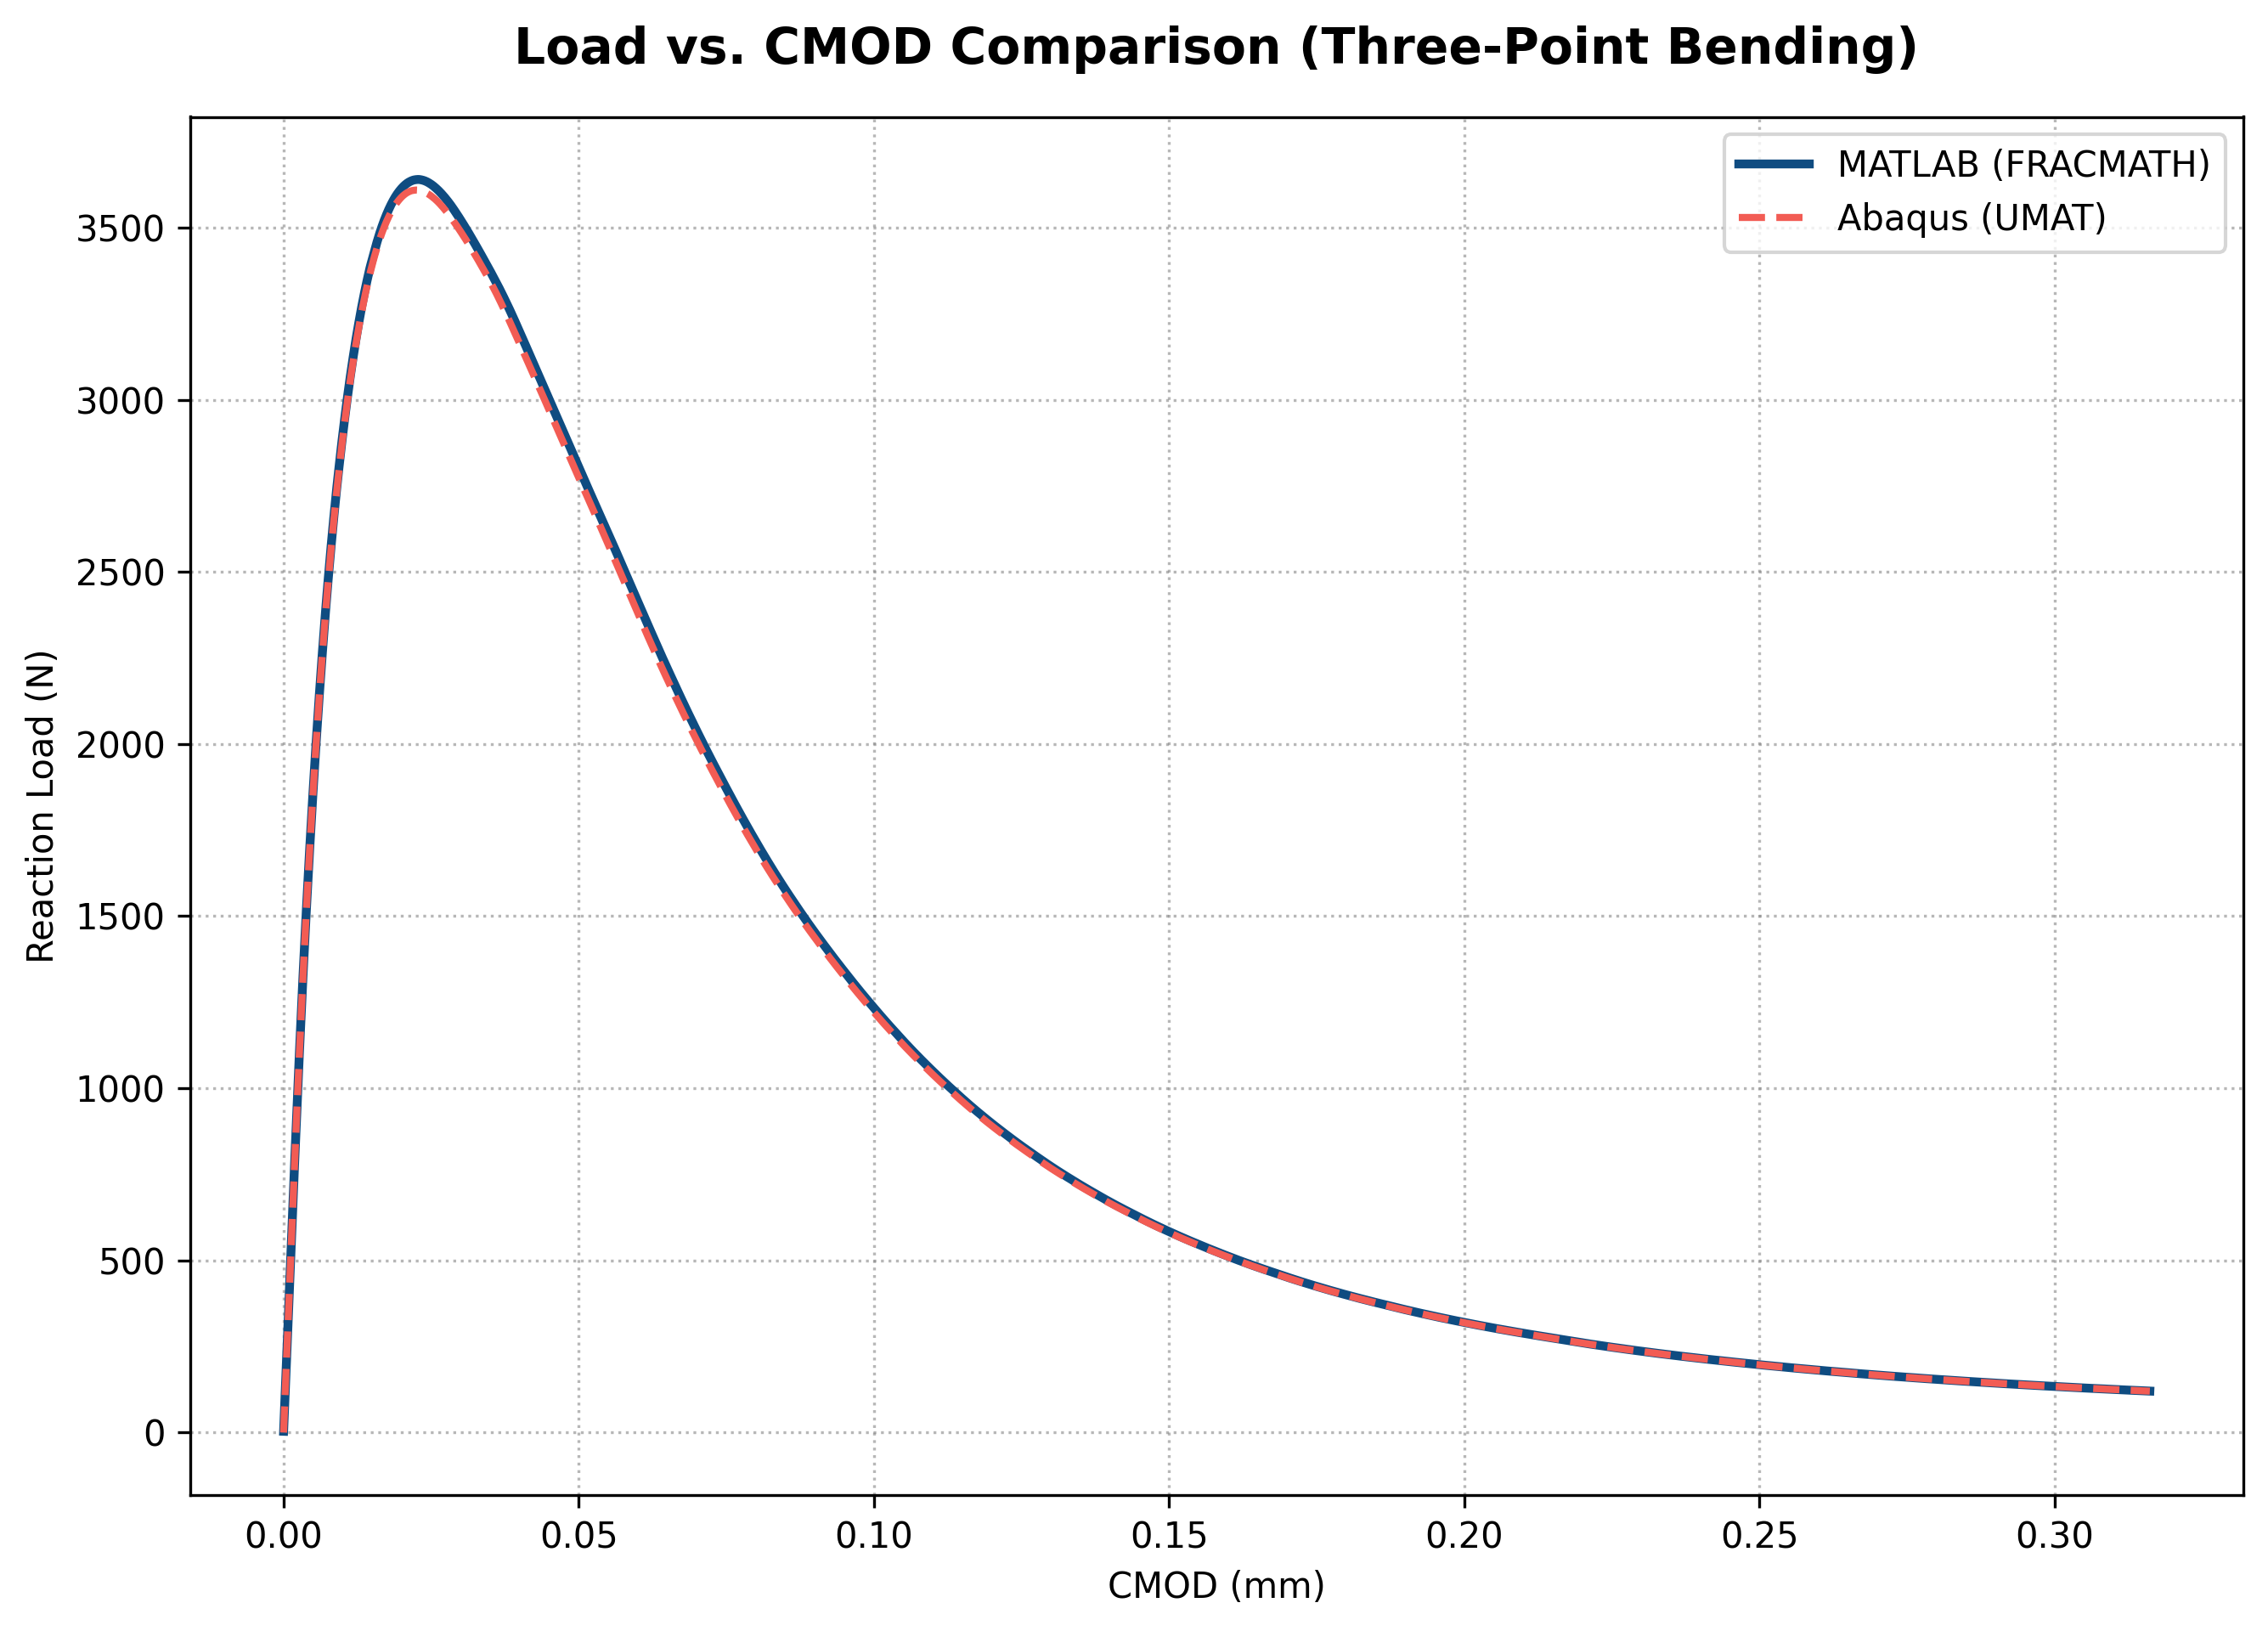
\includegraphics[width=\linewidth]{load_cmod_comparison.png}
    \caption{Load--CMOD response: MATLAB and Oliver-matched Abaqus UMAT.}
  \end{subfigure}
  \caption{Notched 2D three-point bending benchmark. MATLAB and
    Oliver-matched Abaqus UMAT load--CMOD curves track closely up to the
    peak; the post-peak branches remain close but not identical.}
  \label{fig:b1-setup-response}
\end{figure}

\begin{figure}[!htbp]
  \centering
  
\includegraphics[width=\linewidth]{fig_b1_damage.png}

  \vspace{0.2em}
  
\includegraphics[width=\linewidth]{abaqus_fig_damage_last_step.png}

  \caption{Fully damaged bands for the 2D 3PB benchmark: (a) MATLAB peak
    load, 3.64~kN with 17 fully damaged elements; (b) MATLAB post-peak
    state, 0.13~kN at CMOD~$\approx$~0.30~mm with 118 fully damaged
    elements; and (c) Abaqus SDV2 damage field. The MATLAB band grows
    upward from the notch tip; the Abaqus panel marks the damaged crack
    path extracted with the same threshold, $\omega \ge 0.99$.}
  \label{fig:b1-damage}
\end{figure}

For an Oliver-matched check on the crack location and width, the same
case was also run in Abaqus/Standard with the UMAT. The Abaqus
damage variable is stored as SDV2 and is plotted on the undeformed mesh
in Figure~\ref{fig:b1-damage}(c). The black band corresponds to elements
with $\omega \ge 0.99$, which is the same threshold used in the MATLAB
damage figures. With the same mesh, same constitutive law, and same
direction-dependent Oliver bandwidth formula, the relevant comparison is
the predicted crack path, peak response, and post-peak load--CMOD trend.

The wall-clock breakdown of the MATLAB run is given in
Table~\ref{tab:walltime}.

\begin{table}[htbp]
\centering
\caption{MATLAB wall-clock breakdown for the 2D 3PB case
  ($D=100$~mm, $a/D=0.2$).}
\label{tab:walltime}
\begin{tabular}{lrr}
\toprule
Component                     & Time (s) & Share \\
\midrule
Stiffness assembly            & 487.42 & 82.5\% \\
Damage update                 & 12.52  & 2.1\%  \\
Linear solve (UMFPACK)        & 46.81  & 7.9\%  \\
Other (bookkeeping, output)   & 43.79  & 7.4\%  \\
\midrule
\textbf{Total wall clock}     & \textbf{590.54} & \textbf{100\%} \\
\bottomrule
\end{tabular}
\end{table}

At this problem size the sparse direct solve is cheap; the per-element
constitutive update, crack-band length calculation, and sparse assembly
dominate the MATLAB wall-clock cost.

The Abaqus comparison matches the MATLAB solver in geometry, mesh,
loading, boundary conditions, and constitutive law
(Table~\ref{tab:abqcompare}). The UMAT applies the same Oliver bandwidth
of Eq.~\eqref{eq:oliver-t3}, read from the precomputed gradient table
described above, rather than the Abaqus characteristic element length
\texttt{CELENT}.

Small differences remain in the peak load and post-peak branch because
the two codes use different global solution procedures, increment
control, and floating-point operation order.

Figure~\ref{fig:b1-time} compares the wall-clock cost of the two runs.
From the values in Table~\ref{tab:abqcompare},
MATLAB finishes the same benchmark about 3.6 times faster than the
Abaqus/Standard UMAT workflow, and the pie chart shows that MATLAB time
is dominated by assembly rather than by the sparse linear solve.

\begin{figure}[!htbp]
  \centering
  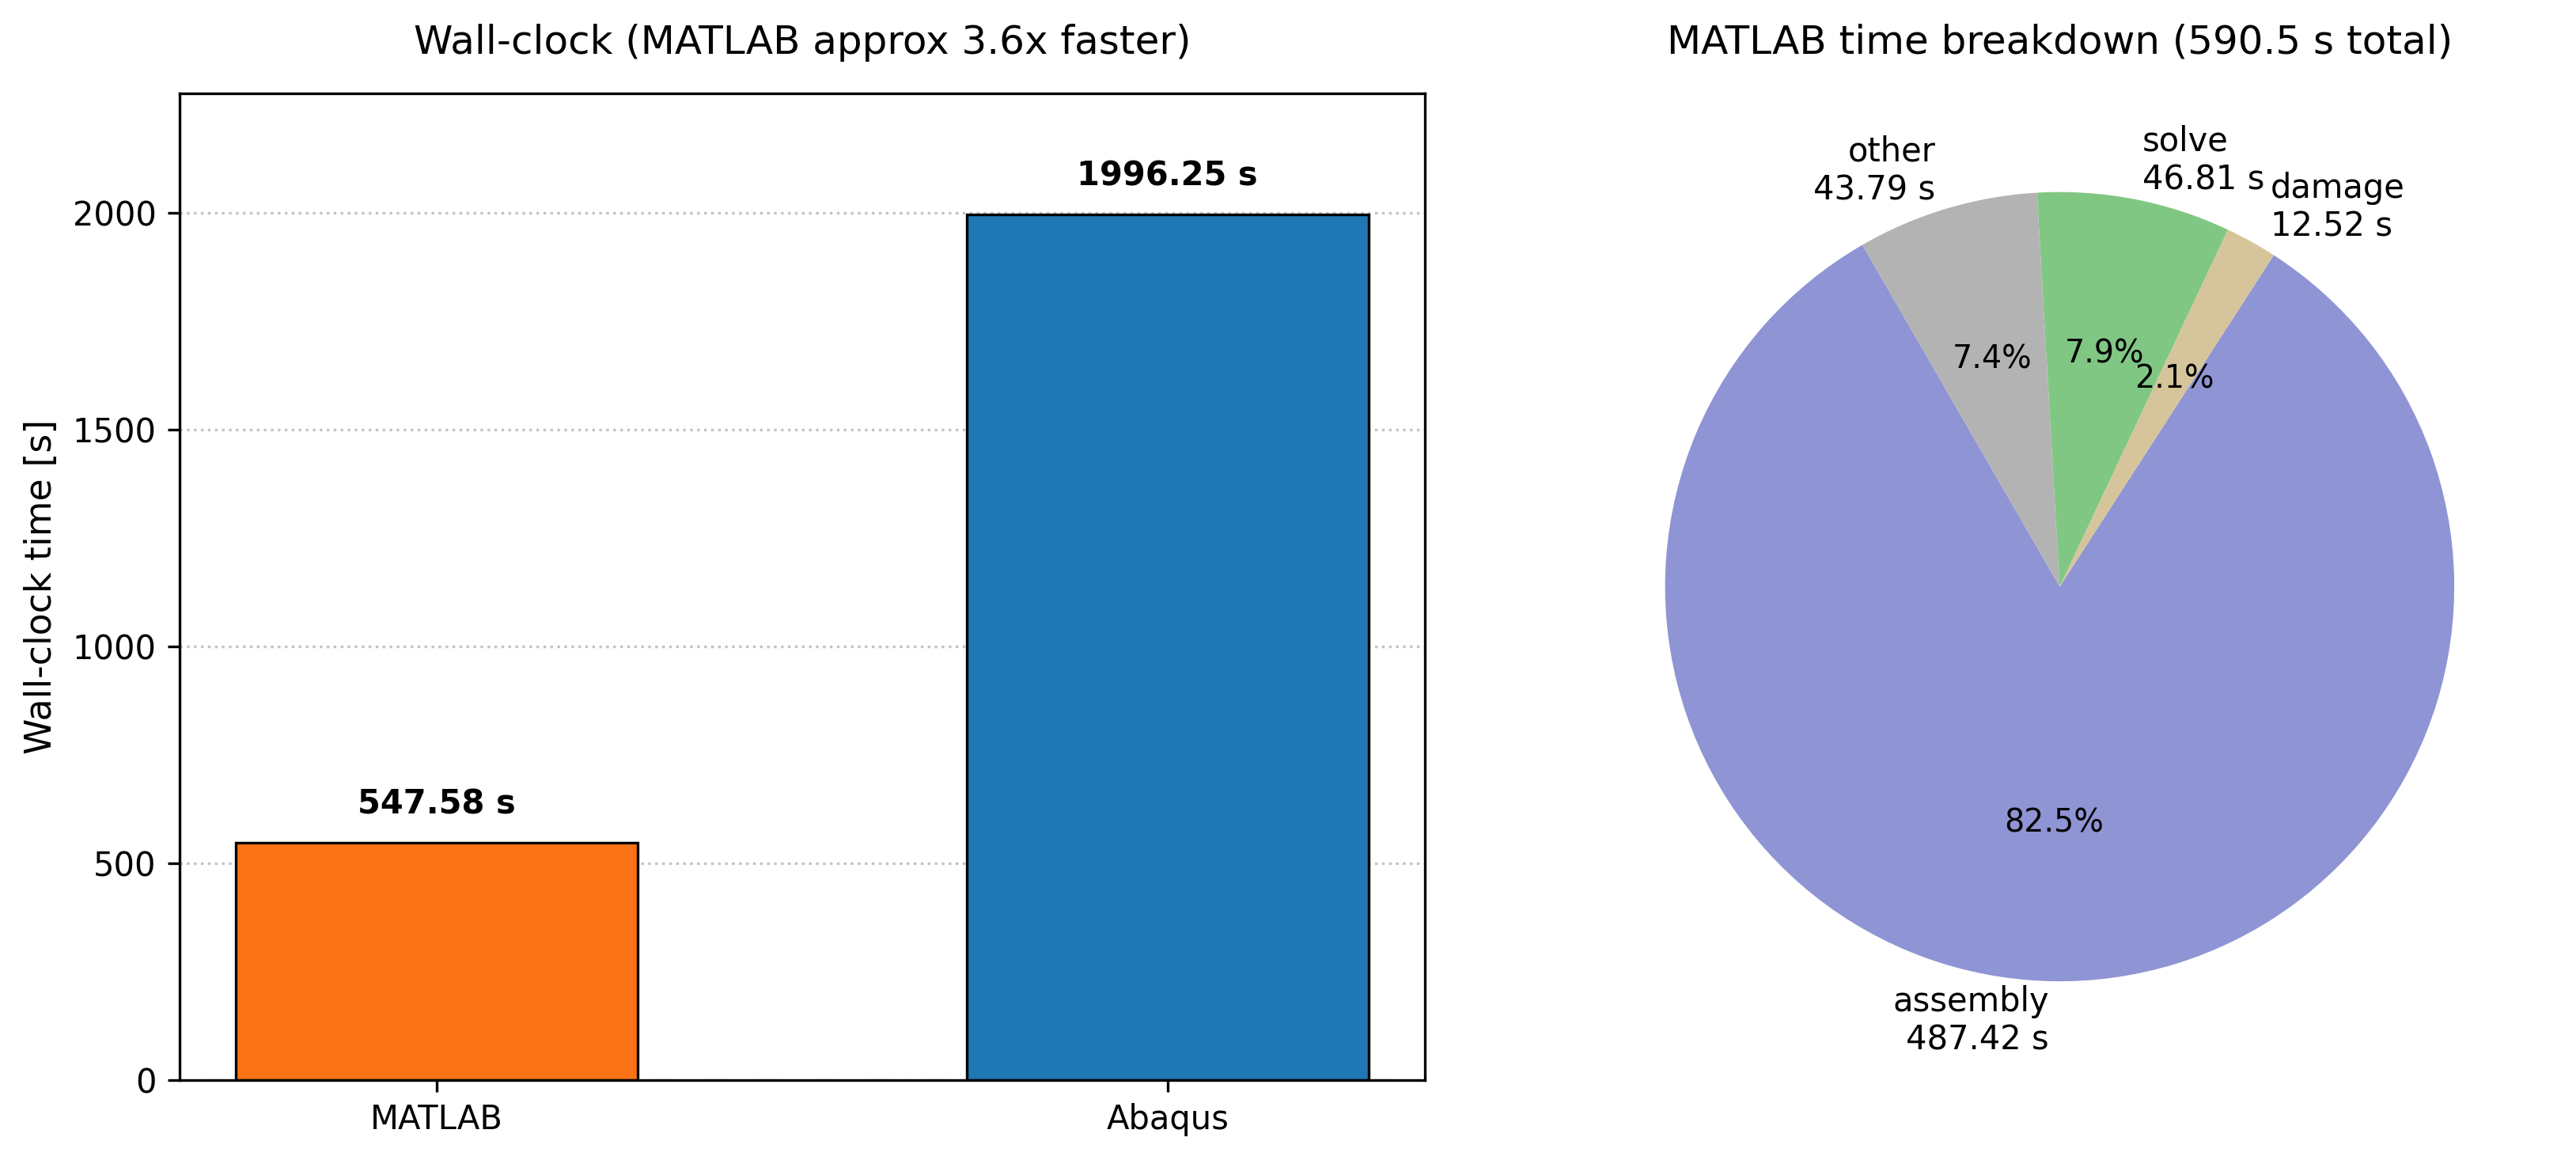
\includegraphics[width=0.95\linewidth]{time_comparison_bar.png}
  \caption{Wall-clock comparison for the 2D 3PB case. Left: total time,
    MATLAB vs.\ Abaqus. Right: the MATLAB time split by component.}
  \label{fig:b1-time}
\end{figure}

\begin{table}[htbp]
\centering
\caption{MATLAB vs.\ Abaqus on the 2D 3PB case using the same geometry,
  mesh, material constants, displacement loading, boundary conditions,
  scalar CDM law, and direction-dependent Oliver T3 crack-band bandwidth.
  MATLAB was run with one thread and Abaqus/Standard was run with four
  threads.}
\label{tab:abqcompare}
\begin{tabular}{lrrr}
\toprule
Quantity & MATLAB & Abaqus + UMAT & Ratio \\
\midrule
Peak load (kN)       & 3.64 & 3.61 & 1.008 \\
CMOD at peak (mm)    & 0.022811 & 0.022485 & 1.015 \\
Wall clock time (s)  & 547.58  & 1996.25 & 0.274 \\
End-to-end/internal time (s) & 590.54 & 1968.00 & 0.300 \\
\bottomrule
\end{tabular}

\vspace{0.4em}
\footnotesize{Values are from the Oliver-matched UMAT comparison.}
\end{table}

% =====================================================================
\subsection*{Benchmark 2: 3D Nooru-Mohamed Mixed Mode Test}
% =====================================================================

The Nooru-Mohamed specimen is a square double edge notched concrete
panel, $200 \times 200 \times 50$~mm, with two horizontal notches 25~mm
long cut from opposite edges at mid height \citep{nooru1992}. The two
notches leave a central ligament that is loaded in a combination of in
plane shear and tension, so its tips experience a genuinely mixed mode
stress state rather than the pure mode I opening of the three point
bending test. We follow load path 4c: a vertical (mode I) displacement is
prescribed on the top edge while a proportional horizontal (shear)
displacement is imposed on the side edges, with a shear to tension ratio
$\gamma = 0.6$, and the bottom edge held fixed. Both components are ramped
together under displacement control over 900 increments to a top
displacement of 0.5~mm. The material is concrete with $E = 29{,}000$~MPa,
$\nu = 0.20$, $f_t = 3.0$~MPa, $G_F = 0.110$~N/mm, and $k = f_c/f_t = 10$
(so $f_c = 30$~MPa).

\begin{figure}[!htbp]
  \centering

  \makebox[\linewidth][c]{%
  \begin{subfigure}{0.52\linewidth}
    \centering
    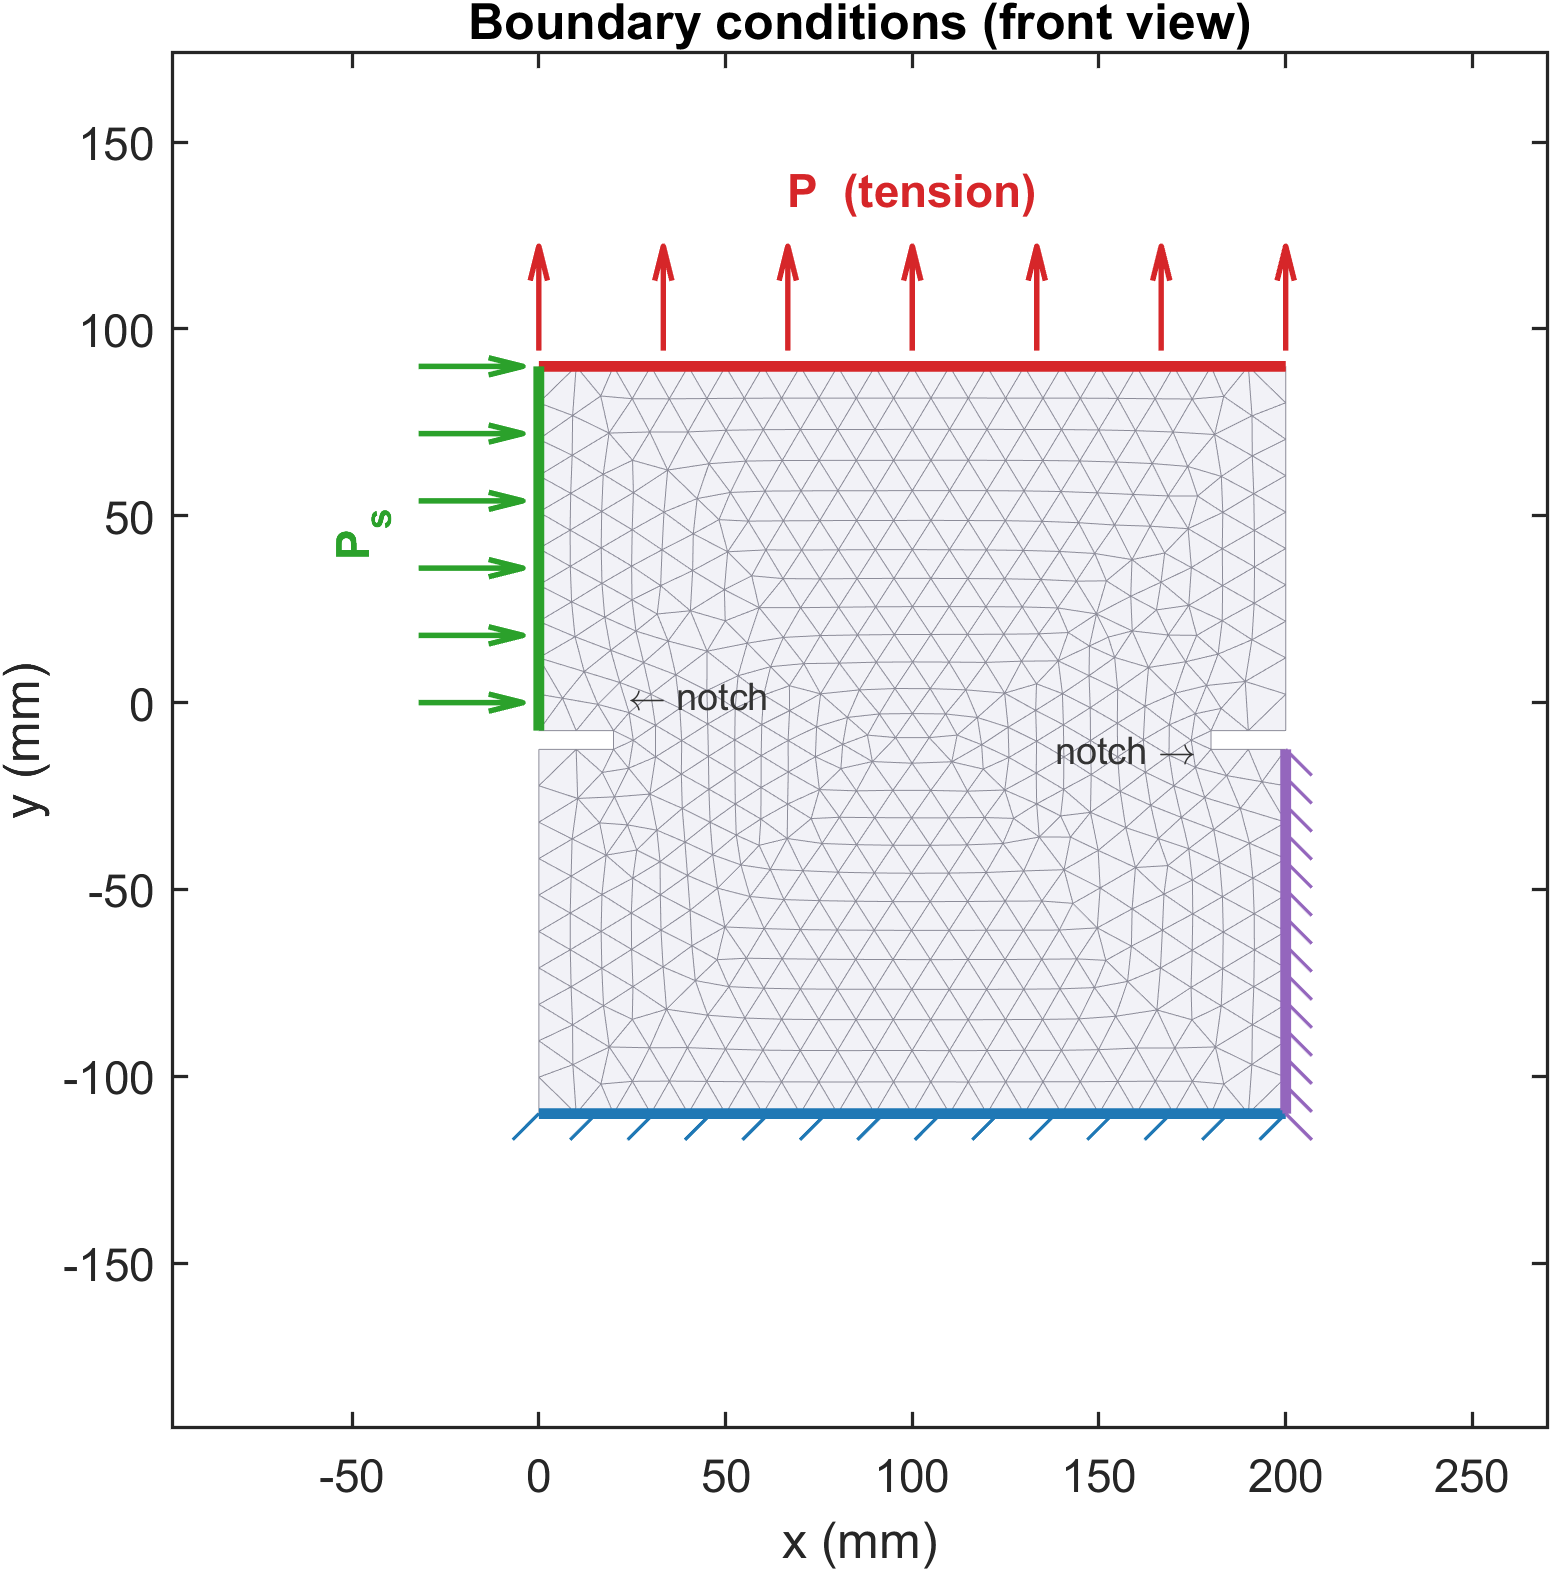
\includegraphics[width=\linewidth]{nooru_BC_2D.png}
    \caption{2D boundary conditions.}
    \label{fig:b2-nooru-bc-2d}
  \end{subfigure}
  \hspace{0.02\linewidth}
  \begin{subfigure}{0.52\linewidth}
    \centering
    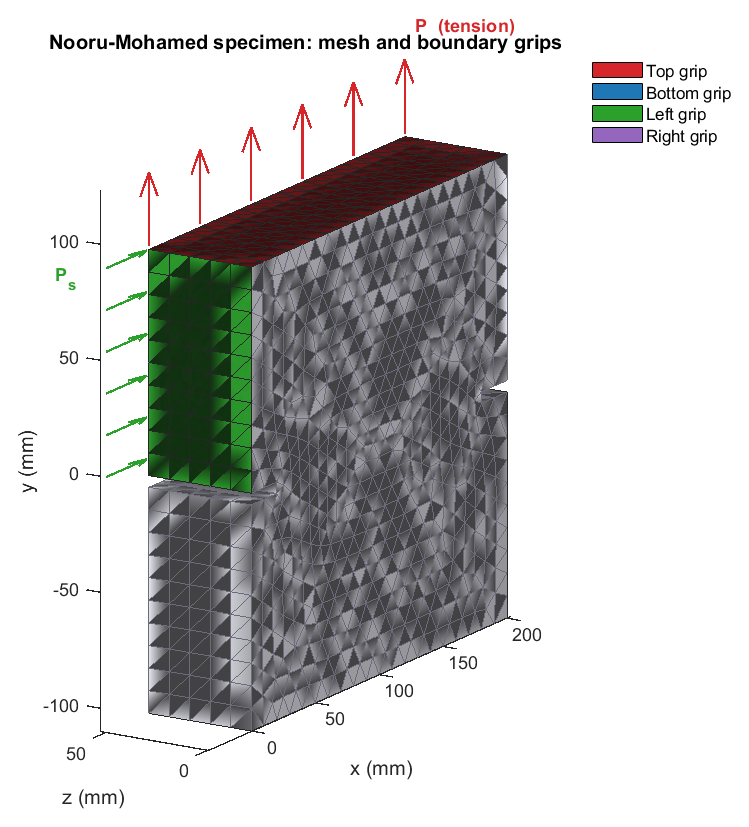
\includegraphics[width=\linewidth]{nooru_mesh_3D_crop.png}
    \caption{3D mesh.}
    \label{fig:b2-nooru-mesh-3d}
  \end{subfigure}}

  \vspace{0.35em}
  \begin{subfigure}{\linewidth}
    \centering
    \makebox[\linewidth][c]{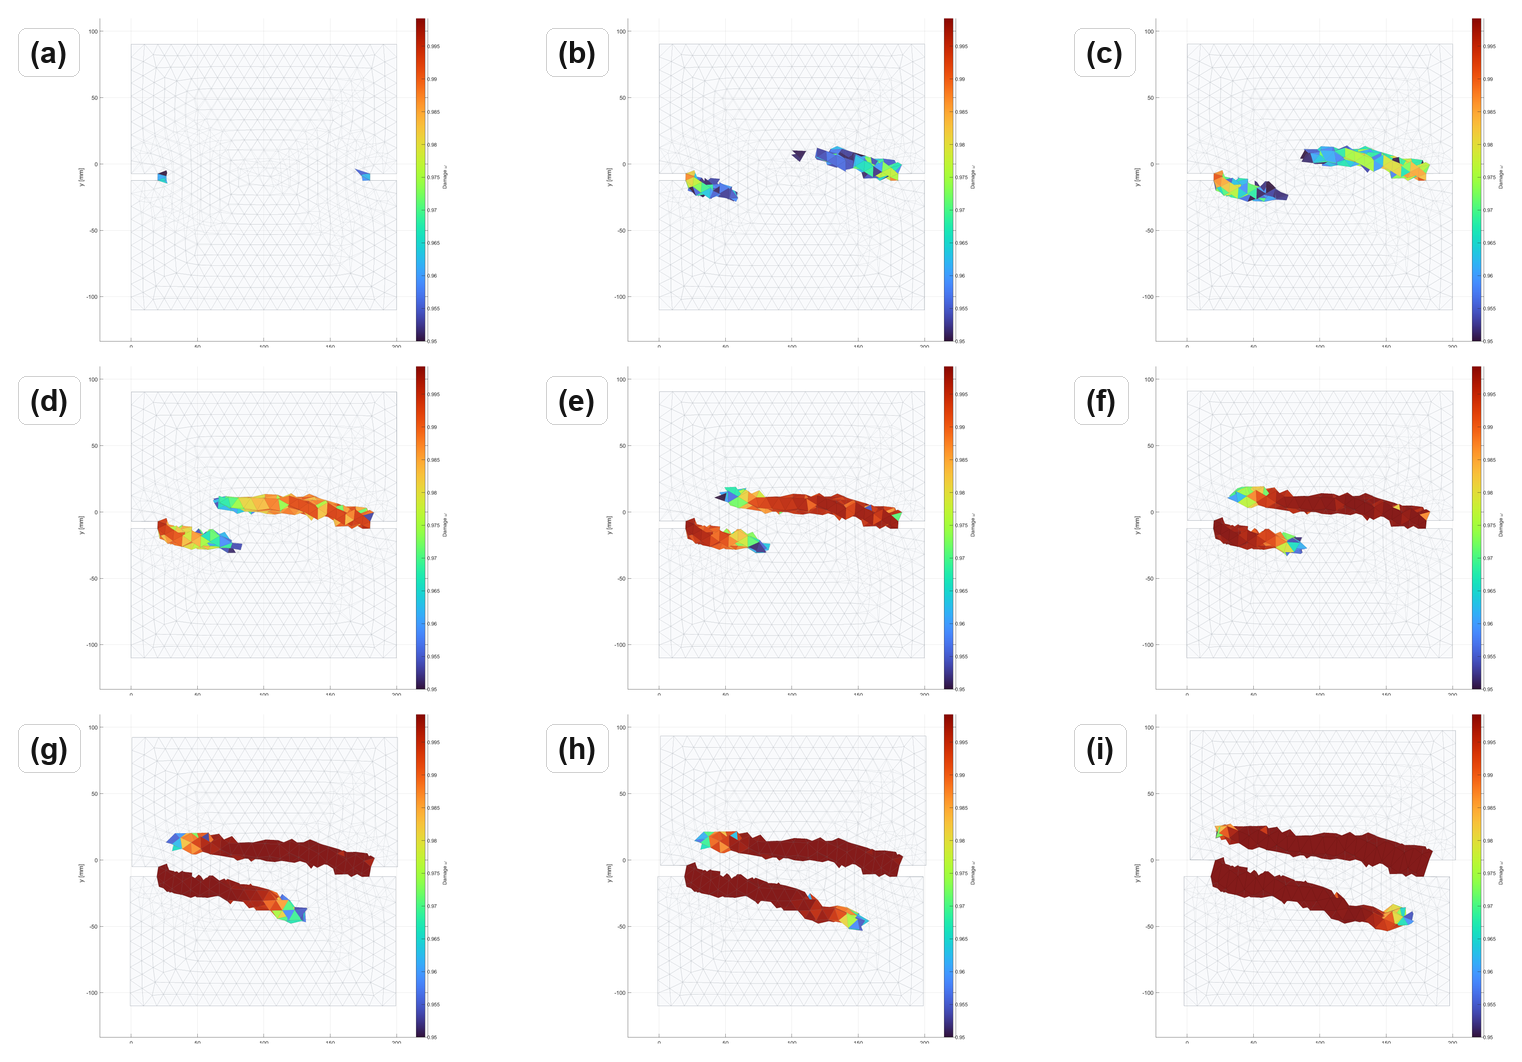
\includegraphics[width=1.12\linewidth]{nooru_damage_evolution_3x3_crop.png}}
    \caption{Damage evolution from first localization at the notches to
      coalescence; panels (a)--(i), left to right and top to bottom,
      correspond to increments 29, 37, 41, 53, 75, 127, 275, 407, and
      900.}
    \label{fig:b2-nooru-damage}
  \end{subfigure}

  \caption{Nooru-Mohamed benchmark: boundary conditions, 3D mesh, and
    damage evolution $\omega$ over the imposed loading history.}
  \label{fig:b2-overview}
\end{figure}

The panel is discretized in full 3D with four node linear tetrahedral
elements (TET4), refined through the ligament between the two notches
where the cracks form and eventually interact; the geometry and the
boundary grips are shown in Figure~\ref{fig:b2-overview}(a,b). The solver is the
same vectorized modified Newton Raphson used for Benchmark~1: a secant
stiffness is assembled from the current damage state at the start of each
load increment and its factorization is reused during the equilibrium
iterations. The same modified von Mises constitutive routine is used, so
nothing in the material model changes between 2D and 3D. The history
variable $\kappa$ is committed once per converged increment, which keeps
the secant system well conditioned as the two bands localize and compete
for the same ligament. Crack band regularization uses Oliver's projected
characteristic length for each tetrahedron. 
Figure~\ref{fig:b2-overview}(c) traces the predicted response from
the first localization at the notch tips (increment~29) through to full
coalescence of the two bands (increment~900). The panels visualize the
full damage field, so both the diffuse process zone and the localized
crack path are visible. The two curved bands and their final separation
reproduce the experimentally observed mixed mode crack pattern; the same
constitutive routine carries over
unchanged from planar mode~I to fully three-dimensional mixed mode
loading.



% =====================================================================
\subsection*{Benchmark 3: 3D Notched Beam Torsion}
% =====================================================================

Brokenshire's torsion test \citep{brokenshire1996,jefferson_torsion} uses a
$400 \times 250 \times 100$~mm plain concrete beam with a diagonal notch
cut through the thickness (depth 25~mm, width 5~mm) across the bottom
face at midspan. In the physical test three supports sit at the bottom
corners and one end of the top edge, and a single point load goes on the
remaining top corner (Figure~\ref{fig:b3-overview}(a)), so the beam is twisted
and the plane of maximum principal tension turns in space around the
notch front, lining up with no face of the mesh. A characteristic length tied to a
fixed mesh direction would lose objectivity here; Oliver's projected
length, recomputed from the local principal direction at each
integration point, keeps the dissipated energy close to $G_F$ for any
crack orientation.

In the model the loaded end is driven directly: one end face is fully
fixed while the opposite end face is given a prescribed rigid-body twist
$\theta$ about the beam axis under rotation control, ramped to
$\theta_{\mathrm{end}} = 3.0\times10^{-3}$~rad over 140 increments. The
reaction torque is recovered from the twisted end, and an equivalent
applied load follows from the lever arm $a = 100$~mm.

The material is plain concrete with $E = 35{,}000$~MPa, $\nu = 0.20$,
$f_t = 3.0$~MPa, $G_F = 0.080$~N/mm ($= 80$~N/m), $\kappa_0 = 6.0\times10^{-5}$,
and $k = f_c/f_t = 10$ (so $f_c = 30$~MPa). Softening is exponential, as
in the other benchmarks, with the softening parameter scaled element by
element through the crack band length.

The mesh is built from four node linear tetrahedral elements (TET4) with
a refined layer around the notch front. The equivalent strain is the same
modified von Mises measure used throughout, and the damage update is
under-relaxed with a factor of 0.35 to keep the staggered fixed point
iteration stable through the steep post-peak branch; each linear solve
reuses a single AMD ordering with a Cholesky factorization. Two points, A
and B, are monitored on opposite sides of the notch at midspan
($x = 200$~mm, $z = \pm 25$~mm), and their relative displacement across
the notch gives the crack opening (Figure~\ref{fig:b3-overview}(a)).

This case is included as a qualitative demonstration of
direction-dependent crack-band regularization under nonplanar,
torsion-driven crack growth. The predicted damage band nucleates at the
notch front and spirals toward the loaded corner
(Figure~\ref{fig:b3-overview}(b--i)), consistent with the fracture
surface observed in the experiment \citep{brokenshire1996}. A
quantitative comparison against the measured load--crack-opening
response is left for the planned nonlocal extension of the framework.

\newcommand{\torsnap}[1]{%
  \includegraphics[width=\linewidth]%
    {Job-1_StaticFast_mod_vm_LIVE_snap_inc_#1.png}}

\begin{figure}[!htbp]
  \centering
  \begin{subfigure}{0.65\linewidth}
    \centering
    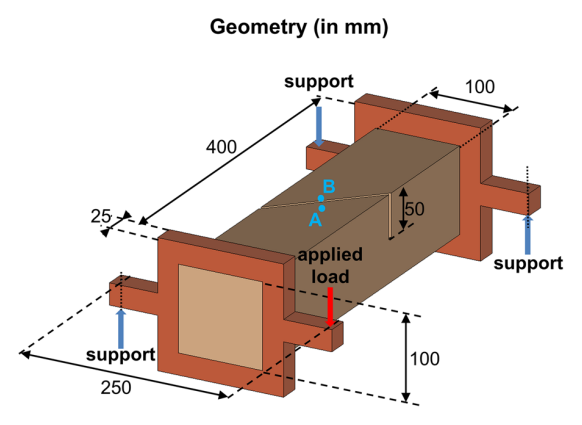
\includegraphics[width=\linewidth]{torsion_crop.png}
    \caption{Brokenshire torsion specimen (mm).}
  \end{subfigure}

  \vspace{0.35em}
  % ---- row 1 ----
  \makebox[\linewidth][c]{%
  \begin{subfigure}{0.33\linewidth}\centering
    \torsnap{0001_theta_2_143e-05}
    \caption{$\theta=2.14\!\times\!10^{-5}$, inc 1}
  \end{subfigure}\hspace{0.01\linewidth}
  \begin{subfigure}{0.33\linewidth}\centering
    \torsnap{0021_theta_4_500e-04}
    \caption{$\theta=4.50\!\times\!10^{-4}$, inc 21}
  \end{subfigure}\hspace{0.01\linewidth}
  \begin{subfigure}{0.33\linewidth}\centering
    \torsnap{0041_theta_8_786e-04}
    \caption{$\theta=8.79\!\times\!10^{-4}$, inc 41}
  \end{subfigure}}

  \vspace{0.35em}
  % ---- row 2 ----
  \makebox[\linewidth][c]{%
  \begin{subfigure}{0.33\linewidth}\centering
    \torsnap{0061_theta_1_307e-03}
    \caption{$\theta=1.31\!\times\!10^{-3}$, inc 61}
  \end{subfigure}\hspace{0.01\linewidth}
  \begin{subfigure}{0.33\linewidth}\centering
    \torsnap{0080_theta_1_714e-03}
    \caption{$\theta=1.71\!\times\!10^{-3}$, inc 80}
  \end{subfigure}\hspace{0.01\linewidth}
  \begin{subfigure}{0.33\linewidth}\centering
    \torsnap{0100_theta_2_143e-03}
    \caption{$\theta=2.14\!\times\!10^{-3}$, inc 100}
  \end{subfigure}}

  \vspace{0.35em}
  % ---- row 3 ----
  \makebox[\linewidth][c]{%
  \begin{subfigure}{0.33\linewidth}\centering
    \torsnap{0120_theta_2_571e-03}
    \caption{$\theta=2.57\!\times\!10^{-3}$, inc 120}
  \end{subfigure}\hspace{0.01\linewidth}
  \begin{subfigure}{0.33\linewidth}\centering
    \torsnap{0140_theta_3_000e-03}
    \caption{$\theta=3.00\!\times\!10^{-3}$, inc 140}
  \end{subfigure}\hspace{0.01\linewidth}
  \begin{subfigure}{0.33\linewidth}\centering
    \phantom{\rule{\linewidth}{0pt}}
  \end{subfigure}}

  \caption{Brokenshire torsion benchmark and damage evolution
    $\omega$ over the imposed twist history. Damage panels are labelled
    by twist $\theta$ and increment; the band nucleates at the notch
    front and spirals toward the loaded corner.}
  \label{fig:b3-overview}
\end{figure}

% =====================================================================
\section*{Impact}
% =====================================================================

\texttt{FRACMATH} is intended to make continuum damage mechanics and
crack-band regularization easier to inspect, modify, and reproduce in a
research workflow. The same scalar damage routine is exercised in a
quantitative 2D Abaqus comparison and in 3D crack-path demonstrations,
so users can study how element-level constitutive updates, projected
bandwidth calculations, sparse assembly, and post-processing interact
without first writing a complete finite element code or a commercial
solver subroutine. The repository includes benchmark inputs, plotting
scripts, result files, smoke tests, and a theory manual so that reviewers
and new users can rerun the examples and compare peak loads, crack paths,
timings, and damage fields.

The package can support new research questions on direction-dependent
crack-band scaling, mesh refinement effects, and MATLAB/Abaqus agreement
for quasibrittle fracture benchmarks. It also provides a reference
implementation for graduate students and early-career researchers who
need a transparent baseline before extending the formulation to nonlocal
damage, anisotropic damage, cyclic loading, or additional element types.

% =====================================================================
\section*{Limitations}
% =====================================================================

The framework is quasistatic, so it includes no inertia and no rate
effects. Damage is treated as isotropic and scalar: a single $\omega$
cannot capture unilateral effects or anisotropic damage under complex
mixed mode loading, which is acceptable for the monotonic loading
considered here but not for cyclic loading. Finally, crack band scaling
delivers mesh objective dissipation but introduces no material length
scale; an integral type or gradient enhanced nonlocal extension is
planned for a later release.

% =====================================================================
\section*{Conclusions}
% =====================================================================

\texttt{FRACMATH} provides a compact MATLAB implementation of scalar CDM
with crack-band regularization, an Oliver-matched Abaqus comparison, and
2D/3D benchmark workflows. The current release is suitable for
reproducible monotonic quasibrittle fracture examples and for method
development within the same framework.

% =====================================================================
\section*{Software availability}
% =====================================================================

Source code, documentation, the benchmark input deck, the Abaqus UMAT,
and a theory manual are available at
\url{https://github.com/Jaykumar9033/FRACMATH} under the MIT license.
The test suite has been verified on MATLAB R2022a, R2023a, and R2024a,
across Linux, macOS, and Windows.

% =====================================================================
\section*{Acknowledgements}
% =====================================================================

The authors acknowledge support from the National Aeronautics and Space
Administration (NASA), and the New Mexico Space Grant Consortium under
grant 80NSSC22M0044.

% =====================================================================
\section*{Declaration of competing interest}
% =====================================================================

The authors declare no conflict of interest.

\section*{Declaration of AI-assisted technologies}

Generative AI tools were used to assist with manuscript wording,
formatting, and implementation support. The scientific claims, equations,
code, numerical results, figures, and references are the responsibility
of the authors.

\section*{Current executable software version}
\label{sec:current-executable-version}

\begin{table}[H]
\centering
\begin{tabular}{|l|p{6.0cm}|p{6.5cm}|}
\hline
\textbf{Nr.} & \textbf{Executable software metadata description} &
\textbf{Value} \\
\hline
S1 & Current executable software version & v1.0.0 \\
\hline
S2 & Permanent link to executable software of this version &
No separate compiled executable; MATLAB source scripts are available in
the GitHub repository. \\
\hline
S3 & Legal Software License & MIT License \\
\hline
S4 & Computing platforms/operating systems & Linux, macOS, and Windows
with MATLAB; Abaqus/Standard is needed only for the UMAT comparison. \\
\hline
\end{tabular}
\caption{Executable software metadata.}
\label{tab:executable-metadata}
\end{table}

\bibliographystyle{elsarticle-num}
\bibliography{paper}

\end{document}
